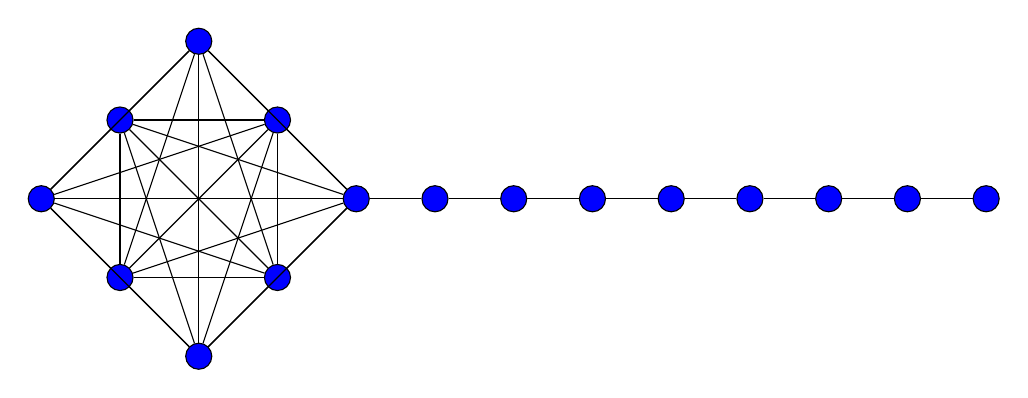
\begin{tikzpicture}
    % Define the 8 vertices in a flat line
    \foreach \i in {1,...,9} {
      \node[draw, fill=blue, circle, minimum size=6pt] (v\i) at (\i, 0) {};
    }
    
    % Draw edges to connect each vertex to the next
    \foreach \i in {1,...,8} {
      \pgfmathtruncatemacro{\j}{\i+1}
      \draw (v\i) -- (v\j);
    }

    % Define additional vertices for the complete graph on v1, centered around v1
    \node[draw, fill=blue, circle, minimum size=6pt] (c1) at (0,1) {};
    \node[draw, fill=blue, circle, minimum size=6pt] (c2) at (0,-1) {};
    \node[draw, fill=blue, circle, minimum size=6pt] (c3) at (-1,2) {};
    \node[draw, fill=blue, circle, minimum size=6pt] (c4) at (-1,-2) {};
    \node[draw, fill=blue, circle, minimum size=6pt] (c5) at (-2,-1) {};
    \node[draw, fill=blue, circle, minimum size=6pt] (c6) at (-2,1) {};
    \node[draw, fill=blue, circle, minimum size=6pt] (c7) at (-3, 0) {};
    
    % Connect the complete graph nodes to v1
    \foreach \k in {1,2,3,4,5,6,7} {
      \draw (v1) -- (c\k);
    }

    % Draw edges between the new nodes to form a complete graph
    \foreach \a in {1,2,3,4,5,6,7} {
      \foreach \b in {\a,...,7} {
        \ifnum\a=\b\else
        \draw (c\a) -- (c\b);
        \fi
      }
    }

  \end{tikzpicture}